\section{Задача 2.1}
\subsection{Задание:}
Вычислить
$
	\dfrac{(2 + 2i)^2 - (1 - i)^3}{(3 + 2i)^3 - (2 + i)^2}
$
\subsection{Решение:}
$
	\dfrac{(2 + 2i)^2 - (1 - i)^3}{(3 + 2i)^3 - (2 + i)^2}
	=
	\dfrac{8i + 2i}{-9 + 46i - 3 - 4i}
	=
	\dfrac{10i}{-12 + 42i}
	=
	\dfrac{35}{159} - \dfrac{17}{159} i
$
\subsection{Проверка в среде Wolfram Mathematica:}
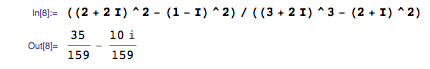
\includegraphics[scale=0.6]{task/2_01/screen1.png}
\subsection{Вывод:}
Мы вычилслили значение выражения и проверили результат в компьютерной среде.
